\section{Connected Graphs}
In order to analyze certain situations that can be modeled by graphs, we must have a better understanding of graphs. As with all areas of mathematics, there is a certain amount of terminology with which we must first be familiar in order to discuss graphs and their properties. Becoming aware of this fundamental terminology is our current goal. First, let's review some concepts and introduce others. Recall that a graph $G$ consists of a finite nonempty set $V$ of vertices and a set $E$ of 2-element subsets of $V$ called edges. If $e = uv$ is an edge of $G$, then the adjacent vertices $u$ and $v$ are said to be \bf{joined} by the edge $e$. The vertices $u$ and $v$ are referred to as \bf{neighbors} of each other. In this case, the vertex $u$ and the edge $e$ (as well as $v$ and $e$) are said to be \bf{incident} with each other. Distinct edges incident with a common vertex are \bf{adjacent edges}.

As we mentioned earlier, although graphs are defined in terms of sets, it is customary and convenient to represent graphs by (and, in fact, to consider them as) diagrams. A graph $G$ with vertex set $V = \{u,v,w,x,y\}$ and edge set $E = \{uv,vw,vx,vy,wy,xy\}$ is shown in Figure 1.15. Since this graph has five vertices and six edges, its order is 5 and its size is 6. In this graph $G$, the vertices $u$ and $v$ are adjacent, while $u$ and $w$ are not adjacent. The vertex $v$ is incident the edge $vw$ but not with the edge $wy$. The edges $uv$ and $vw$ are adjacent, but $uv$ and $xy$ are not adjacent.

\begin{figure}[h]
	\centering
	%G
	\begin{subfigure}[b]{.3\textwidth}
		\centering
		\[G:
		\raisebox{-.5\height}
		{
			\begin{tikzpicture}[scale=.75]
				\vertex (u) at (90:3) [label=right:$u$]{};
				\vertex (v) at (90:1.5) [label=right:$v$]{};
				\vertex (w) at (180:1) [label=left:$w$]{};
				\vertex (x) at (0:1) [label=right:$x$]{};
				\vertex (y) at (270:1.5) [label=below:$y$]{};
				\path
					(u) edge (v)
					(v) edge (w)
					(v) edge (x)
					(v) edge node[right]{$e$} (y)
					(w) edge (y)
					(x) edge node[pos=.4,right]{$e'$} (y)
				;
			\end{tikzpicture}
		}\]
	\end{subfigure}%
	%H
	\begin{subfigure}[b]{.3\textwidth}
		\centering
		\[H:
		\raisebox{-.5\height}
		{
			\begin{tikzpicture}[scale=.75]
				\vertex (v) at (90:1.5) [label=right:$v$]{};
				\vertex (w) at (180:1) [label=left:$w$]{};
				\vertex (x) at (0:1) [label=right:$x$]{};
				\vertex (y) at (270:1.5) [label=below:$y$]{};
				\path
					(v) edge (w)
					(w) edge (y)
					(x) edge (y)
				;
			\end{tikzpicture}
		}\]
	\end{subfigure}%
	%F
	\begin{subfigure}[b]{.3\textwidth}
		\centering
		\[F:
		\raisebox{-.5\height}
		{
			\begin{tikzpicture}[scale=.75]
				\vertex (v) at (90:1.5) [label=right:$v$]{};
				\vertex (w) at (180:1) [label=left:$w$]{};
				\vertex (x) at (0:1) [label=right:$x$]{};
				\path
					(v) edge (w)
					(v) edge (x)
				;
			\end{tikzpicture}
		}\]
	\end{subfigure}
	
	%F'
	\begin{subfigure}[b]{.4\textwidth}
		\centering
		\[F':
		\raisebox{-.5\height}
		{
			\begin{tikzpicture}[scale=.75]
				\vertex (v) at (90:1.5) [label=right:$v$]{};
				\vertex (x) at (0:1) [label=right:$x$]{};
				\vertex (y) at (270:1.5) [label=below:$y$]{};
				\path
					(v) edge node[right]{$e$} (y)
					(x) edge node[pos=.4,right]{$e'$} (y)
				;
			\end{tikzpicture}
		}\]
	\end{subfigure}%
	%G-e
	\begin{subfigure}[b]{.4\textwidth}
		\centering
		\[G-e:
		\raisebox{-.5\height}
		{
			\begin{tikzpicture}[scale=.75]
				\vertex (u) at (90:3) [label=right:$u$]{};
				\vertex (v) at (90:1.5) [label=right:$v$]{};
				\vertex (w) at (180:1) [label=left:$w$]{};
				\vertex (x) at (0:1) [label=right:$x$]{};
				\vertex (y) at (270:1.5) [label=below:$y$]{};
				\path
					(u) edge (v)
					(v) edge (w)
					(v) edge (x)
					(w) edge (y)
					(x) edge (y)
				;
			\end{tikzpicture}
		}\]
	\end{subfigure}
	\caption{A graph $G$ and some of its subgraphs}
\end{figure}

A graph $H$ is called a \bf{subgraph} of a graph $G$, written $H \subseteq G$, if $V(H) \subseteq V(G)$ and $E(H) \subseteq E(G)$. We also say that $G$ contains $H$ as a subgraph. If $H \subseteq G$ and either $V(H)$ is a proper subset of $V(G)$ or $E(H)$ is a proper subset of $E(G)$, then $H$ is a \bf{proper subgraph} of $G$. So the graph $H$ of Figure 1.15 is a subgraph of the graph $G$ shown in that figure; indeed, $H$ is a proper subgraph of $G$. If a subgraph of a graph $G$ has the same vertex set as $G$, then it is a \bf{spanning subgraph} of $G$.

A subgraph $F$ of a graph $G$ is called an \bf{induced subgraph} of $G$ if whenever $u$ and $v$ are vertices of $F$ and $uv$ is an edge of $G$, then $uv$ is an edge of $F$ as well. Therefore, the graph $H$ of Figure 1.15 is not an induced subgraph of the graph $G$ of Figure 1.15 since, for example, $v,x \in V(H)$ and $vx \in E(G)$ but $vx \centernot\in E(H)$. On the other hand, the graph $F$ of Figure 1.15 is an induced subgraph of $G$. If $S$ is a nonempty set of vertices of a graph $G$, then the \bf{subgraph of} $G$ \bf{induced by} $S$ is the induced subgraph with vertex set $S$. This induced subgraph is denoted by $G[S]$. For a nonempty set $X$ of edges, the \bf{subgraph} $G[X]$ \bf{induced by} $X$ has edge set $X$ and consists of all vertices that are incident with at least one edge in $X$. This subgraph is called an \bf{edge-induced subgraph} of $G$. Sometimes $\langle S \rangle_{G}$ and $\langle X \rangle_{G}$ are used for $G[S]$ and $G[X]$, respectively. The graph $F'$ of Figure 1.15 is an edge-induced subgraph of $G$ in that figure; indeed, $F' = G[X']$, where $X' = \{e,e'\}$.

Any proper subgraph of a graph $G$ can be obtained by removing vertices and edges from $G$. For an edge $e$ of $G$, we write $G-e$ for the spanning subgraph of $G$ whose edge set consists of all edges of $G$ except $e$. More generally, if $X$ is a set of edges of $G$, then $G-X$ is the spanning subgraph of $G$ with $E(G-X) = E(G) \smallsetminus X$. For the graph $G$ of Figure 1.15 and $e = vy$, the subgraph $G - e$ is shown. If $X = \{e_{1},e_{2},\ldots,e_{k}\}$, then we also write $G-X$ as $G-e_{1}-e_{2}-\cdots-e_{k}$.

For a vertex $v$ of a nontrivial graph $G$, the subgraph $G-v$ consists of all vertices of $G$ except $v$ and all edges of $G$ except those incident with $v$. For a proper subset $U$ of $V(G)$, the subgraph $G-U$ has vertex set $V(G) \smallsetminus U$ and its edge set consists of all edges of $G$ joining two vertices in $V(G) \smallsetminus U$. Necessarily, $G-U$ is an induced subgraph of $G$. For $U = \{u,y\}$ in the graph $G$ of Figure 1.15, $G-U$ is the subgraph $F$ shown in that figure.

If $u$ and $v$ are nonadjacent vertices of a graph $G$, then $e = uv \centernot\in E(G)$. By $G+e$, we mean the graph with vertex set $V(G)$ and edge set $E(G) \union \{e\}$. Thus $G$ is a spanning subgraph of $G+e$.

Many of the concepts that occur in graph theory and which we will investigate in detail later concern various ways in which one can "move about" in a graph. In particular, if we think of the vertices of a graph as locations and the edges as roads between certain pairs of locations, then the graph can be considered as modeling some community. There is a variety of kinds of trips that can be taken in the community.

Let's start at some vertex $u$ of a graph $G$. If we proceed from $u$ to a neighbor of $u$ and then to a neighbor of that vertex and so on, until we finally come to a stop at a vertex $v$, then we have just described a walk from $u$ to $v$ in $G$. More formally, a $u-v$ \bf{walk} $W$ in $G$ is a sequence of vertices in $G$, beginning with $u$ and ending at $v$ such that consecutive vertices in the sequence are adjacent, that is, we can express $W$ as
\begin{equation}
W = (u=v_{0},v_{1},\ldots,v_{k}=v),
\end{equation}
where $k \geq 0$ and $v_{i}$ and $v_{i+1}$ are adjacent for $i = 0,1,2,\ldots,k-1$. Each vertex $v_{i}$ $(0 \leq i \leq k)$ and each edge $v_{i}v_{i+1}$ $(0 \leq i \leq k-1)$ is said to lie on or belong to $W$. Notice that the definition of the walk $W$ does not require the listed vertices to be distinct; in fact, even $u$ and $v$ are not required to be distinct. However, every two consecutive vertices in $W$ are distinct since they are adjacent. If $u=v$, then the walk $W$ is \bf{closed}; while if $u \neq v$, then $W$ is \bf{open}. As we move from one vertex of $W$ to the next, we are actually encountering or traversing edges of $G$, possibly traversing some edges of $G$ more than once. The number of edges encountered in a walk (including multiple occurrences of an edge) is called the \bf{length} of the walk. Thus the length of the walk $W$ defined in (1.1) is $k$.

For the graph $G$ of Figure 1.16,
\begin{equation}
W = (x,y,w,y,v,w)
\end{equation}
is therefore a walk, indeed an $x-w$ walk of length 5 (one less than the number of occurrences of vertices in the walk). A walk of length 0 is a \bf{trivial walk}. So $W = (v)$ is a trivial walk. (By this definition, those people who feel guilty about not exercising need not feel guilty any longer as going for a daily "walk" just became easier.)

Provided we continue to proceed from a vertex to one of its neighbors (and eventually stop), there is essentially no conditions on a walk. However, there will be occasions when we want to place restrictions on certain types of walks.

\begin{figure}[h]
	\[G:
	\raisebox{-.5\height}
	{
		\begin{tikzpicture}[x=1.5cm,y=1.5cm]
			\foreach \i/\j in {1/u, 0/v, 2/x, 3/y} {
				\setcounter{Angle}{45 + \i * 360 / 4};
				\vertex (\j) at (\theAngle:1) [label=\theAngle:$\j$]{};
			}
			\vertex (w) at (0,0) [label=above:$w$]{};
			\path
				(u) edge (v)
				(u) edge (w)
				(v) edge (w)
				(v) edge (y)
				(w) edge (x)
				(w) edge (y)
				(x) edge (y)
			;
		\end{tikzpicture}
	}\]
	\caption{Illustrating walks in a graph}
\end{figure}

Borrowing terminology from the Old West, we define a $u-v$ \bf{trail} in a graph $G$ to be a $u-v$ walk in which no edge is traversed more than once. Thus, the $x-w$ walk $W$ in (1.2) is \it{not} an $x-w$ trail as the edge $wy$ is repeated. On the other hand,
\begin{equation}
T = (u,w,y,x,w,v)
\end{equation}
is a $u-v$ trail in the graph $G$ of Figure 1.16. Notice that this trail $T$ repeats the vertex $w$. This is perfectly permissible. Although the definition of a trail stipulates that no edge can be repeated, no such condition is placed on vertices.

A $u-v$ walk in a graph in which no vertices are repeated is a $u-v$ \bf{path}. While the $u-v$ trail $T$ in (1.3) is not a $u-v$ path in the graph $G$ of Figure 1.16 (since the vertex $w$ is repeated),
\begin{align*}
P = (u,w,y,v)
\end{align*}
\it{is} a $u-v$ path. If no vertex in a walk is repeated (thereby producing a path), then no edge is repeated either. Hence every path is a trail.

If a $u-v$ walk in a graph is followed by a $v-w$ walk, then a $u-w$ walk results. In particular, a $u-v$ path followed by a $v-w$ path is a $u-w$ walk $W$ but not necessarily a $u-w$ path, as vertices in $W$ may be repeated. While not every walk is a path, if a graph contains a $u-v$ walk, then it must also contain a $u-v$ path. This is our first theorem.

\begin{thm}
If a graph $G$ contains a $u-v$ walk of length $l$, then $G$ contains a $u-v$ path of length at most $l$.
\end{thm}

\begin{pf}
Among all $u-v$ walks in $G$, let
\begin{align*}
P = (u = u_{0},u_{1},\ldots,u_{k} = v)
\end{align*}
be a $u-v$ walk of smallest length $k$. Therefore, $k \leq l$. We claim that $P$ is a $u-v$ path. Assume, to the contrary, that this is not the case. Then some vertex of $G$ must be repeated in $P$, say $u_{i} = u_{j}$ for some $i$ and $j$ with $0 \leq i < j \leq k$. If we then delete the vertices $u_{i+1},u_{i+2},\ldots,u_{j}$ from $P$, we arrive at the $u-v$ walk
\begin{align*}
(u = u_{0},u_{1},\ldots,u_{i-1},u_{i} = u_{j},u_{j+1},\ldots,u_{k} = v)
\end{align*}
whose length is less than $k$, which is impossible. Therefore, as claimed, $P$ is a $u-v$ path of length $k \leq l$.
\end{pf}

A \bf{circuit} in a graph $G$ is a closed trail of length 3 or more. Hence a circuit begins and ends at the same vertex but repeats no edges. A circuit can be described by choosing any of its vertices as the beginning (and ending) vertex provided the vertices are listed in the same cyclic order. In a circuit, vertices can be repeated, in addition to the first and last. For example, in the graph $G$ of Figure 1.16,
\begin{equation}
C = (y,w,u,v,w,x,y) \text{ or } C = (x,y,w,u,v,w,x) \text{ or } C = (w,x,y,w,u,v,w)
\end{equation}
is a circuit. A circuit that repeats no vertex, except for the first and last, is a \bf{cycle}. A $k$\bf{-cycle} is a cycle of length $k$. A 3-cycle is also referred to as a \bf{triangle}. A cycle of odd length is called an \bf{odd cycle}; while, not surprisingly, a cycle of even length is called an \bf{even cycle}. In the graph $G$ of Figure 1.16, the circuit $C$ in (1.4) is not a cycle, while
\begin{align*}
C' = (x,y,v,w,x)
\end{align*}
\it{is} a cycle, namely a 4-cycle. If a vertex of a cycle is deleted, then a path is obtained. This is not necessarily true for circuits, however.

The vertices and edges of a trail, path, circuit or cycle in a graph $G$ form a subgraph of $G$, also called a \bf{trail}, \bf{path}, \bf{circuit} or \bf{cycle}. Hence a path, for example, is used to describe both a manner of traversing certain vertices and edges of $G$ and a subgraph consisting of those vertices and edges. The graph $G$ of Figure 1.16 is shown again in Figure 1.17. Thus the subgraphs $G_{1}, G_{2}, G_{3}, G_{4}$ of the graph $G$ are a trail, path, circuit and cycle, respectively.

\begin{figure}[h]
	\centering
	%G
	\begin{subfigure}[b]{.3\textwidth}
		\[G:
		\raisebox{-.5\height}
		{
			\begin{tikzpicture}[x=1.5cm,y=1.5cm]
				\foreach \i/\j in {1/u, 0/v, 2/x, 3/y} {
					\setcounter{Angle}{45 + \i * 360 / 4};
					\vertex (\j) at (\theAngle:1) [label=\theAngle:$\j$]{};
				}
				\vertex (w) at (0,0) [label=above:$w$]{};
				\path
					(u) edge (v)
					(u) edge (w)
					(v) edge (w)
					(v) edge (y)
					(w) edge (x)
					(w) edge (y)
					(x) edge (y)
				;
			\end{tikzpicture}
		}\]
	\end{subfigure}%
	%G1
	\begin{subfigure}[b]{.3\textwidth}
		\[G_{1}:
		\raisebox{-.5\height}
		{
			\begin{tikzpicture}[x=1.5cm,y=1.5cm]
				\foreach \i/\j in {1/u, 0/v, 2/x, 3/y} {
					\setcounter{Angle}{45 + \i * 360 / 4};
					\vertex (\j) at (\theAngle:1) [label=\theAngle:$\j$]{};
				}
				\vertex (w) at (0,0) [label=above:$w$]{};
				\path
					(u) edge (w)
					(v) edge (w)
					(w) edge (x)
					(w) edge (y)
					(x) edge (y)
				;
			\end{tikzpicture}
		}\]
	\end{subfigure}%
	%G2
	\begin{subfigure}[b]{.3\textwidth}
		\[G_{2}:
		\raisebox{-.5\height}
		{
			\begin{tikzpicture}[x=1.5cm,y=1.5cm]
				\foreach \i/\j in {1/u, 0/v, 3/y} {
					\setcounter{Angle}{45 + \i * 360 / 4};
					\vertex (\j) at (\theAngle:1) [label=\theAngle:$\j$]{};
				}
				\vertex (w) at (0,0) [label=above:$w$]{};
				\path
					(u) edge (w)
					(v) edge (y)
					(w) edge (y)
				;
			\end{tikzpicture}
		}\]
	\end{subfigure}
	
	%G3
	\begin{subfigure}[b]{.4\textwidth}
		\[G_{3}:
		\raisebox{-.5\height}
		{
			\begin{tikzpicture}[x=1.5cm,y=1.5cm]
				\foreach \i/\j in {1/u, 0/v, 2/x, 3/y} {
					\setcounter{Angle}{45 + \i * 360 / 4};
					\vertex (\j) at (\theAngle:1) [label=\theAngle:$\j$]{};
				}
				\vertex (w) at (0,0) [label=above:$w$]{};
				\path
					(u) edge (v)
					(u) edge (w)
					(v) edge (w)
					(w) edge (x)
					(w) edge (y)
					(x) edge (y)
				;
			\end{tikzpicture}
		}\]
	\end{subfigure}%
	%G4
	\begin{subfigure}[b]{.4\textwidth}
		\[G_{4}:
		\raisebox{-.5\height}
		{
			\begin{tikzpicture}[x=1.5cm,y=1.5cm]
				\foreach \i/\j in {0/v, 2/x, 3/y} {
					\setcounter{Angle}{45 + \i * 360 / 4};
					\vertex (\j) at (\theAngle:1) [label=\theAngle:$\j$]{};
				}
				\vertex (w) at (0,0) [label=above:$w$]{};
				\path
					(v) edge (w)
					(v) edge (y)
					(w) edge (x)
					(x) edge (y)
				;
			\end{tikzpicture}
		}\]
	\end{subfigure}
	\caption{Trails, paths, circuits and cycles as subgraphs of a graph}
\end{figure}

We will have a special interest in graphs $G$ in which it is possible to travel from each vertex of $G$ to any other vertex of $G$. If $G$ contains a $u-v$ path, then $u$ and $v$ are said to be \bf{connected} and $u$ \bf{is connected to} $v$ (and $v$ is connected to $u$). So, saying that $u$ and $v$ are connected only means that there is some $u-v$ path in $G$; it doesn't say that $u$ and $v$ are joined by an edge. Of course, if $u$ \it{is} joined to $v$, then $u$ is connected to $v$ as well. A graph $G$ is \bf{connected} if every two vertices of $G$ are connected, that is, if $G$ contains a $u-v$ path for every pair $u,v$ of vertices of $G$. By Theorem 1.6, G is connected if and only if G contains a $u-v$ walk for every pair $u,v$ of vertices of $G$. Since every vertex is connected to itself, the trivial graph is connected.

A graph $G$ that is not connected is \bf{disconnected}. A connected subgraph of $G$ that is not a proper subgraph of any other connected subgraph of $G$ is a \bf{component} of $G$. The number of components of a graph $G$ is denoted by $k(G)$. Thus a graph $G$ is connected if and only if $k(G) = 1$. While the graph $G$ of Figure 1.16 is connected, the graph $H$ of Figure 1.18 is disconnected since, for example, there is no $s-w$ path in $H$. There is no $x-z$ path either. The graph $H$ has three components, namely $H_{1}$, $H_{2}$ and $H_{3}$ and so $k(H) = 3$.

For subgraphs $G_{1},G_{2},\ldots,G_{k}$, $k \geq 2$, of a graph $G$, with mutually disjoint vertex sets, we write $G = G_{1} \union G_{2} \union \ldots \union G_{k}$ if every vertex and every edge of $G$ belong to exactly one of these subgraphs. In this case, $G$ is the \bf{union} of the graphs $G_{1},G_{2},\ldots,G_{k}$. In particular, we write $G = G_{1} \union G_{2} \union \ldots \union G_{k}$ if $G_{1},G_{2},\ldots,G_{k}$ are components of $G$. That is, every graph is the union of its components. Therefore, we can write $H = H_{1} \union H_{2} \union H_{3}$ for the graphs in Figure 1.18.

\begin{figure}[h]
	\centering
	%H=H1 U H2 U H3
	\begin{subfigure}[b]{.9\textwidth}
		\[H = H_{1} \union H_{2} \union H_{3}:
		\raisebox{-.5\height}
		{
			\begin{tikzpicture}
				\vertex (s) at (0,1) [label=left:$s$]{};
				\vertex (t) at (1,1) [label=right:$t$]{};
				\vertex (u) at (0,0) [label=left:$u$]{};
				\vertex (v) at (1,0) [label=right:$v$]{};
				\vertex (w) at (2,1) [label=below:$w$]{};
				\vertex (x) at (3,1) [label=below:$x$]{};
				\vertex (y) at (4,1) [label=below:$y$]{};
				\vertex (z) at (5,1) [label=below:$z$]{};
				\path
					(s) edge (t)
					(s) edge (u)
					(t) edge (v)
					(u) edge (v)
					(w) edge (x)
					(x) edge (y)
				;
			\end{tikzpicture}
		}\]
	\end{subfigure}
	
	%H1
	\begin{subfigure}[b]{.3\textwidth}
		\[H_{1}:
		\raisebox{-.5\height}
		{
			\begin{tikzpicture}
				\vertex (s) at (0,1) [label=left:$s$]{};
				\vertex (t) at (1,1) [label=right:$t$]{};
				\vertex (u) at (0,0) [label=left:$u$]{};
				\vertex (v) at (1,0) [label=right:$v$]{};
				\path
					(s) edge (t)
					(s) edge (u)
					(t) edge (v)
					(u) edge (v)
				;
			\end{tikzpicture}
		}\]
	\end{subfigure}%
	%H2
	\begin{subfigure}[b]{.3\textwidth}
		\[H_{2}:
		\raisebox{-.5\height}
		{
			\begin{tikzpicture}
				\vertex (w) at (0,1) [label=below:$w$]{};
				\vertex (x) at (1,1) [label=below:$x$]{};
				\vertex (y) at (2,1) [label=below:$y$]{};
				\path
					(w) edge (x)
					(x) edge (y)
				;
			\end{tikzpicture}
		}\]
	\end{subfigure}%
	%H3
	\begin{subfigure}[b]{.3\textwidth}
		\[H_{3}:
		\raisebox{-.5\height}
		{
			\begin{tikzpicture}
				\vertex (z) at (0,1) [label=below:$z$]{};
			\end{tikzpicture}
		}\]
	\end{subfigure}
	\caption{A disconnected graph and its components}
\end{figure}

Components can also be defined by means of an equivalence relation. (Equivalence relations are reviewed in Appendix B.1.)

\begin{thm}
Let $R$ be the relation defined on the vertex set of a graph $G$ by $u R v$, where $u,v \in V(G)$, if $u$ is connected to $v$, that is if $G$ contains a $u-v$ path. Then $R$ is an equivalence relation.
\end{thm}

\begin{pf}
It is immediate that $R$ is reflexive and symmetric. It remains therefore only to show that $R$ is transitive. Let $u,v,w \in V(G)$ such that $u R v$ and $v R w$. Hence $G$ contains a $u-v$ path $P'$ and a $v-w$ path $P''$. As we have seen earlier, following $P'$ by $P''$ produces a $u-w$ walk $W$. By Theorem 1.6, $G$ contains a $u-w$ path and so $u R w$.
\end{pf}

The equivalence relation described in Theorem 1.7 produces a partition of the vertex set of every graph $G$ into equivalence classes. The subgraph of $G$ induced by the vertices in an equivalence class is a component of $G$. Exercise 1.14 asks you to show this. As a consequence, we have the following:
\begin{cons}
Each vertex and each edge of a graph $G$ belong to exactly one component of $G$. This implies that if $G$ is a disconnected graph and $u$ and $v$ are vertices belonging to different components of $G$, then $uv \centernot\in E(G)$.
\end{cons}

The following theorem provides a sufficient condition for a graph of order at least 3 to be connected.

\begin{thm}
Let $G$ be a graph of order 3 or more. If $G$ contains two distinct vertices $u$ and $v$ such that $G-u$ and $G-v$ are connected, then $G$ itself is connected.
\end{thm}

\begin{pf}
Suppose that $G$ contains distinct vertices $u$ and $v$ such that $G-u$ and $G-v$ are connected. To show that $G$ itself is connected, we show that every two vertices of $G$ are connected. Let $x$ and $y$ be two vertices of $G$. We consider two cases.

\it{Case 1. $\{x,y\} \neq \{u,v\}$, say $u \centernot\in \{x,y\}$.} Then $x$ and $y$ are vertices in $G-u$. Since $G-u$ is connected, there is an $x-y$ path $P$ in $G-u$. Hence $P$ is in $G$ and $x$ and $y$ are connected in $G$.

\it{Case 2. $\{x,y\} = \{u,v\}$, say $x = u$ and $y = v$.} We show that $u$ and $v$ are connected in $G$. Since the order of $G$ is at least 3, there is a vertex $w$ in $G$ such that $w \neq u,v$. Since $G-v$ is connected, $G-v$ contains a $u-w$ path $P'$. Furthermore, since $G-u$ is connected, $G-u$ contains a $w-v$ path $P''$. Therefore, $P'$ followed by $P''$ produces a $u-v$ walk. By Theorem 1.6, $G$ contains a $u-v$ path and so $u$ and $v$ are connected in $G$.
\end{pf}

If $G$ is the disconnected graph consisting of two vertices $u$ and $v$ and no edges, then the subgraphs $G-u$ and $G-v$ are (trivially) connected. Therefore, in Theorem 1.8, it is essential that the order of the graph under consideration be at least 3.

If $u$ and $v$ are vertices in a connected graph $G$, then there must be a $u-v$ path in $G$. However, it is quite possible that $G$ contains several $u-v$ paths. For example, in the graph $G$ of Figure 1.16, all of the following are $u-y$ paths:
\begin{align*}
P' = (u,v,y) && P'' = (u,w,v,y) && P''' = (u,v,w,x,y).
\end{align*}
The length of $P'$ is 2, the length of $P''$ is 3 and the length of $P'''$ is 4. There is no $u-y$ path of length 1 in this graph since $u$ and $y$ are not adjacent and there are no $u-y$ paths of length 5 or more as $G$ only has five vertices.

Let $G$ be a connected graph of order $n$ and let $u$ and $v$ be two vertices of $G$. The \bf{distance} between $u$ and $v$ is the smallest length of any $u-v$ path in $G$ and is denoted by $d_{G}(u,v)$ or simply $d(u,v)$ if the graph $G$ under consideration is clear. Hence if $d(u,v)=k$, then there exists a $u-v$ path
\begin{equation}
P = (u = v_{0},v_{1},\ldots,v_{k} = v)
\end{equation}
of length $k$ in $G$ but no $u-v$ path of smaller length exists in $G$. A $u-v$ path of length $d(u,v)$ is called a $u-v$ \bf{geodesic}. In fact, since the path $P$ in (1.5) is a $u-v$ geodesic, not only is $d(u,v)=d(u,v_{k})=k$ but $d(u,v_{i})=i$ for every $i$ with $0 \leq i \leq k$. Exercise 1.16 asks you to verify this. If $u=v$, then $d(u,v)=0$. If $uv \in E(G)$, then $d(u,v)=1$. In general, $0 \leq d(u,v) \leq n-1$ for every two vertices $u$ and $v$ (distinct or not) in a connected graph of order $n$. For the vertices $u$ and $y$ in the graph $G$ of Figure 1.16, $d(u,y)=2$. If $G$ is disconnected, then there are some pairs $x,y$ of distinct vertices of $G$ such that there is no $x-y$ path in $G$. In this case, $d(x,y)$ is not defined.

At times, it is useful to visualize the vertices of a connected graph according to their distances from a given vertex. The graph $H$ of Figure 1.19(a) is redrawn in Figure 1.19(b) to indicate those vertices at a given distance from the vertex $t$. The vertex $t$ (the only vertex whose distance from $t$ is 0) is drawn at the top. The vertices one level down are the neighbors of $t$. The next level consists of those vertices whose distance from $t$ is 2 and so on. Observe that two adjacent vertices must either belong to the same level or neighboring levels.

\begin{figure}[h]
	\centering
	\begin{subfigure}[b]{.4\textwidth}
		\[H:
		\raisebox{-.5\height}
		{
			\begin{tikzpicture}
				\vertex (q) at (1,2) [label=above:$q$]{};
				\vertex (r) at (2,2) [label=above:$r$]{};
				\vertex (s) at (3,2) [label=above:$s$]{};
				\fvertex (t) at (0,1) [label=left:$t$]{};
				\vertex (u) at (1,1) [label=135:$u$]{};
				\vertex (v) at (2,1) [label=45:$v$]{};
				\vertex (w) at (3,1) [label=right:$w$]{};
				\vertex (x) at (0,0) [label=below:$x$]{};
				\vertex (y) at (1,0) [label=below:$y$]{};
				\vertex (z) at (2,0) [label=below:$z$]{};
				\path
					(q) edge (r)
					(q) edge (u)
					(r) edge (s)
					(r) edge (u)
					(r) edge (v)
					(s) edge (w)
					(t) edge (u)
					(t) edge (x)
					(u) edge (v)
					(u) edge (x)
					(u) edge (y)
					(v) edge (w)
					(v) edge (z)
					(x) edge (y)
					(y) edge (z)
				;
			\end{tikzpicture}
		}\]
		\caption{}
	\end{subfigure}%
	\begin{subfigure}[b]{.4\textwidth}
		\[\raisebox{-.5\height}
		{
			\begin{tikzpicture}
				\vertex (q) at (0,1) [label=left:$q$]{};
				\vertex (r) at (1,1) [label=135:$r$]{};
				\vertex (s) at (.5,0) [label=below:$s$]{};
				\fvertex (t) at (1.5,3) [label=above:$t$]{};
				\vertex (u) at (1,2) [label=left:$u$]{};
				\vertex (v) at (2,1) [label=right:$v$]{};
				\vertex (w) at (1.5,0) [label=below:$w$]{};
				\vertex (x) at (2,2) [label=right:$x$]{};
				\vertex (y) at (3,1) [label=right:$y$]{};
				\vertex (z) at (2.5,0) [label=below:$z$]{};
				\draw[dotted] (.5,1.75)--(.5,2.25)--(2.5,2.25)--(2.5,1.75)--cycle;
				\draw[dotted] (-.5,.75)--(-.5,1.25)--(3.5,1.25)--(3.5,.75)--cycle;
				\draw[dotted] (0,-.25)--(0,.25)--(3,.25)--(3,-.25)--cycle;
				\path
					(q) edge (r)
					(q) edge (u)
					(r) edge (s)
					(r) edge (u)
					(r) edge (v)
					(s) edge (w)
					(t) edge (u)
					(t) edge (x)
					(u) edge (v)
					(u) edge (x)
					(u) edge (y)
					(v) edge (w)
					(v) edge (z)
					(x) edge (y)
					(y) edge (z)
				;
			\end{tikzpicture}
		}\]
		\caption{}
	\end{subfigure}
	\caption{Distances from a given vertex}
\end{figure}

The greatest distance between any two vertices of a connected graph $G$ is called the \bf{diameter} of $G$ and is denoted by $diam(G)$. The diameter of the graph $H$ of Figure 1.19 is 3. The path $P' = (y,u,r,s)$ is a $y-s$ geodesic whose length is $diam(H)$.

If $G$ is a connected graph such that $d(u,v) = diam(G)$ and $w \neq u,v$, then no $u-w$ geodesic can contain $v$, for otherwise $d(u,w) > d(u,v) = diam(G)$, which is impossible.

Let's return to Theorem 1.8, where we proved that if a graph $G$ of order 3 contains two distinct vertices $u$ and $v$ such that $G-u$ and $G-v$ are connected, then $G$ is connected. Actually, the converse of this theorem is also true; that is, if $G$ is a connected graph of order at least 3, then $G$ must contain two vertices $u$ and $v$ such that $G-u$ and $G-v$ are both connected. We are now in a position to prove this theorem as well.

\begin{thm}
If $G$ is a connected graph of order 3 or more, then $G$ contains two distinct vertices $u$ and $v$ such that $G-u$ and $G-v$ are connected.
\end{thm}

\begin{pf}
Let $u$ and $v$ be two vertices of $G$ such that $d(u,v) = diam(G)$. We claim that $G-u$ and $G-v$ are both connected. Suppose that this is not the case. Then at least one of $G-u$ and $G-v$ is disconnected, say $G-v$ is disconnected. Therefore, $G-v$ contains two vertices $x$ and $y$ that are not connected in $G-v$. However, since $G$ is connected, the vertices $u$ and $x$ are connected in $G$, as are $u$ and $y$.

Let $P'$ be an $x-u$ geodesic in $G$ and $P''$ be a $u-y$ geodesic in $G$. Since $d_{G}(u,v) = diam(G)$, the vertex $v$ cannot lie on either $P'$ or on $P''$, so $P'$ and $P''$ are paths in $G-v$. The path $P'$ followed by $P''$ produces an $x-y$ walk $W$ in $G-v$. By Theorem 1.6, $G-v$ contains an $x-y$ path and so $x$ and $y$ are connected in $G-v$. This is a contradiction.
\end{pf}

Theorem 1.9 gives a property that every connected graph of order at least 3 must have. That is, Theorem 1.9 provides a \it{necessary condition} for a graph to be connected. Actually, Theorem 1.9 is true even if the order of $G$ is 2, but we stated Theorem 1.9 as we did so we could combine Theorems 1.8 and 1.9 into a single \it{necessary and sufficient condition} for a graph to be connected, which we state next.

\begin{thm}
Let $G$ be a graph of order 3 or more. Then $G$ is connected if and only if $G$ contains two distinct vertices $u$ and $v$ such that $G-u$ and $G-v$ are connected.
\end{thm}

\begin{exers}\end{exers}

\begin{exer}
Let $G$ be the graph of Figure 1.20, let $X = \{e,f\}$, where $e = ru$ and $f = vw$, and let $U = \{u,w\}$. Draw the subgraphs $G-X$ and $G-U$ of $G$.

\begin{figure}[h]
	\centering
	\[G:
	\raisebox{-.5\height}
	{
		\begin{tikzpicture}
			\vertex (r) at (0,2) [label=left:$r$]{};
			\vertex (s) at (1,2) [label=above:$s$]{};
			\vertex (t) at (2,2) [label=right:$t$]{};
			\vertex (u) at (0,1) [label=left:$u$]{};
			\vertex (v) at (1,1) [label=315:$v$]{};
			\vertex (w) at (2,1) [label=right:$w$]{};
			\vertex (x) at (0,0) [label=left:$x$]{};
			\vertex (y) at (1,0) [label=below:$y$]{};
			\vertex (z) at (2,0) [label=right:$z$]{};
			\path
				(r) edge (s)
				(r) edge (u)
				(r) edge (v)
				(s) edge (t)
				(s) edge (v)
				(t) edge (v)
				(t) edge (w)
				(u) edge (v)
				(u) edge (x)
				(v) edge (w)
				(v) edge (y)
				(w) edge (z)
				(x) edge (y)
				(y) edge (z)
			;
		\end{tikzpicture}
	}\]
	\caption{The graph $G$ in Exercises 1.11 and 1.12}
\end{figure}
\end{exer}

\begin{exer}
For the graph $G$ of Figure 1.20, give an example of each of the following or explain why no such example exists.
\begin{enumerate}[{(a)}]
\item An $x-y$ walk of length 6.
\item A $v-w$ trail that is not a $v-w$ path.
\item An $r-z$ path of length 2.
\item An $x-z$ path of lenth 3.
\item An $x-t$ path of length $d(x,t)$.
\item A circuit of length 10.
\item A cycle of length 8.
\item A geodesic whose length is $diam(G)$.
\end{enumerate}
\end{exer}

\begin{exer}
\begin{enumerate}[{(a)}]
\item Give an example of a connected graph $G$ containing three vertices $u$,$v$ and $w$ such that $d(u,v)=d(u,w)=d(v,w)=diam(G)=3$.
\item Does the question in (a) suggest another question?
\end{enumerate}
\end{exer}

\begin{exer}
For a graph $G$, a component of $G$ has been defined as (1) a connected subgraph of $G$ that is not a proper subgraph of any other connected subgraph of $G$ and has been described as (2) a subgraph of $G$ induced by the vertices in an equivalence class resulting from the equivalence relation defined in Theorem 1.7. Show that these two interpretations of components are equivalent.
\end{exer}

\begin{exer}
Draw all connected graphs of order 5 in which the distance between two distinct vertices is odd. Explain why you know that you have drawn all such graphs.
\end{exer}

\begin{exer}
Let $P = (u = v_{0},v_{1},\ldots,v_{k} = v)$, $k \geq 1$, be a $u-v$ geodesic in a connected graph $G$. Prove that $d(u,v_{i}) = i$ for each integer $i$ with $1 \leq i \leq k$.
\end{exer}

\begin{exer}
\begin{enumerate}[{(a)}]
\item Prove that if $P$ and $Q$ are two longest paths in a connected graph, then $P$ and $Q$ have at least one vertex in common.
\item Prove or disprove: Let $G$ be a connected graph of diameter $k$. If $P$ and $Q$ are two geodesics of length $k$ in $G$, then $P$ and $Q$ have at least one vertex in common.
\end{enumerate}
\end{exer}

\begin{exer}
A graph $G$ of order 12 has vertex set $V(G) = \{c_{1},c_{2},\ldots,c_{12}\}$ for the twelve configurations in Figure 1.4. A "move" on this checkerboard corresponds to moving a single coin to an unoccupied square, where
\begin{enumerate}[{(1)}]
\item the gold coin can only be moved horizontally or diagonally,
\item the silver coin can only be moved vertically or diagonally,
\end{enumerate}
Two vertices $c_{i}$ and $c_{j}$ $(i \neq j)$ are adjacent if it is possible to move $c_{i}$ to $c_{j}$ by a single move.
\begin{enumerate}[{(a)}]
\item What vertices are adjacent to $c_{1}$ in $G$?
\item What vertices are adjacent to $c_{2}$ in $G$?
\item Draw the subgraph of $G$ induced by $\{c_{2},c_{6},c_{9},c_{11}\}$.
\item Give an example of a $c_{1}-c_{7}$ path in $G$.
\end{enumerate}
\end{exer}

\begin{exer}
Theorem 1.10 states that a graph $G$ of order 3 or more is connected if and only if $G$ contains two distinct vertices $u$ and $v$ such that $G-u$ and $G-v$ are connected. Based on this, one might suspect that the following statement is true. \it{Every connected graph $G$ of order 4 or more contains three distinct vertices $u$, $v$ and $w$ such that $G-u$, $G-v$ and $G-w$ are connected.} Is it?
\end{exer}

\begin{exer}
\begin{enumerate}[{(a)}]
\item Let $u$ and $v$ be distinct vertices in a connected graph $G$. There may be several connected subgraphs of $G$ containing $u$ and $v$. What is the minimum size of a connected subgraph of $G$ containing $u$ and $v$? Explain your answer.
\item Does the question in (a) suggest another question to you?
\end{enumerate}
\end{exer}